\section{Implementation details and hyper-parameters}
\label{app:sec:implementation}

\subsection{\svdacro training}
We obtain the expert vectors $z$ as the base components in \implname by training the \svdacro fine-tunes with a consistent recipe across the considered training tasks and language models. 
We divide each dataset to produce equal-sized training and validation splits. We then apply our RL-based approach, optimizing $\theta_z$ with AdamW using a learning rate of $2 \times 10^{-3}$ with cosine decay, a batch size of 256, and gradient clipping. 
We employ early stopping and select the best $\lambda$ (the coefficient of the KL divergence term) based on validation performance. For the \llamaXL and Vision tasks experiments, we apply the \svdacro on half of the layers to reduce memory usage while maintaining considerable performance improvement.
During the training of \llama on the vision language tasks, we apply a small negative reward (-0.1) for training stability.

\subsection{LoRA training}
\begin{wrapfigure}{h}{0.55\textwidth}
  \centering
  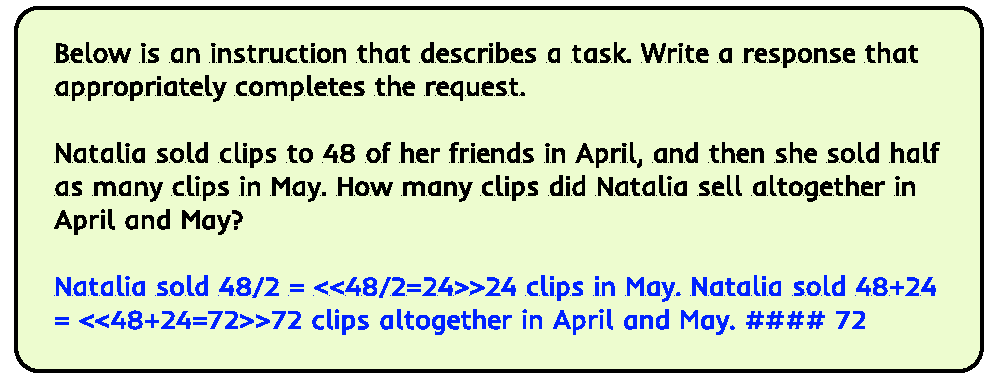
\includegraphics[width=\linewidth]{images/visualization/ift_math_example.pdf}
   \vspace{-6mm}
  \caption{\textbf{Sample problem and answer.} Math data sample used for LoRA instruction fine-tuning, text in blue is the unmasked solution.}
  \label{app:fig:sft_math_example}
\end{wrapfigure}

We follow community best practices for LoRA fine-tuning, applying it to query and value projection layers with learning rates around $5 \times 10^{-5}$. 
We set 200 total iterations with a 256 global batch size for sufficient training. For feasible LoRA instruction training, we collect solutions for all training tasks (GSM8K, MBPP, Arc-Easy, TextVQA) from official sources and append them to question prompts. 
Table~\ref{app:fig:sft_math_example} shows a sample math problem used for LoRA fine-tuning.
Despite extensive hyperparameter tuning, we often observe test performance decay as discussed, which can be attributed to the small number of training samples and potential model requirements for instruction fine-tuning data (specifically, the highly detailed thinking process).

\subsection{Hyper parameters}
We present a summary of the hyperparameters used in our experiments in Table~\ref{app:tab:hyperparameters}. To optimize performance, we conducted sweeps across several hyperparameters and selected the most effective combination based on validation results.
For \svdacro, our primary focus was on adjusting the KL coefficient to enhance training stability. In the case of LoRA, we concentrated on sweeping the learning rate and maximum gradient clip norm to identify optimal settings.

\begin{table}[!h]
\centering
\caption{\textbf{Hyper-parameters used for \svdacro and LoRA training.} We perform a sweep on certain sensitive hyper-parameters  across methods for fair comparison.}
% \vspace{-3.5mm}
\begin{tabular}{ll}
\toprule
\multicolumn{2}{c}{\textbf{\svdacro Hyperparameters}} \\
\midrule
Initial mean value of $z$ & $0.1$ \\
Initial variance value of $z$ & $1 \times 10^{-3}$ \\
Global batch size & $256$ \\
Learning rate & $2 \times 10^{-3}$ \\
Clip max norm & $1 \times 10^{-3}$ \\
KL coefficient $\lambda$ & $0.0$, $0.1$, $0.2$, $0.3$ \\
\midrule
\multicolumn{2}{c}{\textbf{LoRA Hyperparameters}} \\
\midrule
Rank & $16$ \\
LoRA alpha & $32$ \\
LoRA dropout & $0.05$ \\
Global batch size & $256$ \\
Learning rate & $1 \times 10^{-5}$, $5 \times 10^{-5}$, $1 \times 10^{-4}$ \\
Clip max norm & $1 \times 10^{-3}$, $1.0$ \\
\bottomrule
\end{tabular}
\label{app:tab:hyperparameters}
\end{table}

\subsection{Few-shot adaptation}
\label{app:sec:fewshot}

As described in the main text, our few-shot adaptation approach entails producing an entirely new $z^\prime=\sum^{K}_{k=1} \alpha_k z_k$ for each $W$ by linearly interpolating between the $K$ learned \svdacro vectors, each weighted by the coefficients $\alpha \in \mathbb{R}^K$.
We employ CEM to search for $\alpha_k$'s based on the performance on the few-shot prompts, which are specifically held out from the rest of the test prompts and used to obtain the elite set at each iteration. 
In the case of multiple sample solutions obtaining the same score on these held-out samples, we break ties by choosing the sample solution with the highest average log-likelihood across the tokens of its generated correct answers.

In all of our main experiments, we reserve only 10 samples of data for self-adaptation and perform up to 100 CEM iterations. For each setting, we consider both per-layer and per-vector adaptation, where the latter strategy has the advantage of greatly simplifying search (as we only have 3 $\alpha$ coefficients). Moreover, we experiment with both normalizing across the $\alpha$ of different tasks (such that their sum would be fixed to 1) or keeping them unconstrained. Due to the lack of a validation set, we simply report the performance attained by our best sample from these test configurations at the end of optimization, on the remaining unseen samples for each task.
